\chapter{Methode}
In dit hoofdstuk wordt het ontwerp en de realisatie van de ontworpen pipet besproken. Hierbij worden de verschillende onderdelen behandeld, als ook de gemaakte keuzes.
\section{Conceptueel ontwerp}
\subsection{Literatuurstudie}
De Literatuurstudie bestond voor een groot deel uit het bestuderen van beschikbare patenten. Patenten zoals\ \cite{RN16} en\ \cite{RN17} beschrijven analoge pipetten. Deze worden nog manueel bediend en hebben een relatief eenvoudige werking. Deze patenten waren belangrijk om de basiswerking van moderne pipetten te begrijpen. Ze tonen namelijk aan dat deze pipetten met één eenvoudige zuigerwerking werken. Dit is een belangrijke stap bij het ontwerp van de automatische pipet.
\\\textit{Zie \autoref{sec: Analoge pipetten} voor verdere toelichting betreffende de werking.}
\\[12pt]Verder werden de patenten \ \cite{RN35},\ \cite{RN36} en\ \cite{RN38} bestudeerd. Deze patenten beschrijven de werking van een, motorisch aangedreven, elektronische pipet. In het geval van\ \cite{RN36} en\ \cite{RN38} wordt niet toegelicht welk type motor gebruikt wordt. In het geval van\ \cite{RN35} wordt er vermeld dat er voor een stappermotor is gekozen. Deze patenten tonen aan dat de zuigerwerking van een pipet met een stappermotor kan gebeuren en dat deze met een hoge precisie kunnen werken. Ook dit is een belangrijke stap in het ontwerp van de automatische pipet.
\section{Hardware ontwerp}
Zoals eerder vernoemd is voor het hardware ontwerp gekozen voor een modulaire oplossing. Dit laat toe om de verschillende onderdelen onafhankelijk van elkaar te ontwikkelen en indien nodig aan te passen. Dit maakt het in de toekomst ook mogelijk om dit ontwerp uit te breiden tot bijvoorbeeld een meerkanaals systeem.
\\[12pt]De verschillende modules worden geplaatst over geleidestaven, zoals in\ \autoref{fig:geleidestaven} te zien is. Deze geleidestaven zorgen ervoor dat de verschillende modules op een vaste plaats blijven staan. 

\begin{figure}
    \centering
    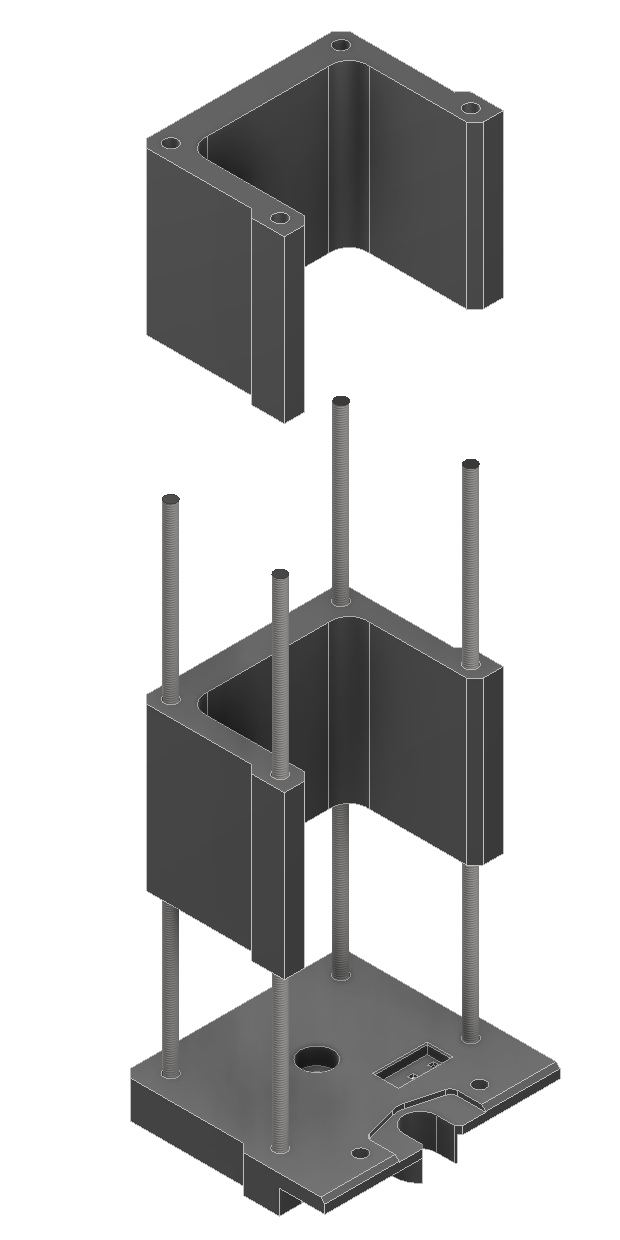
\includegraphics[width=.4\textwidth]{figures/GuidesDemonstration.png}
    \caption{Demonstartie van de geleidestaven.}\label{fig:geleidestaven}
\end{figure}%
\begin{figure}
    \centering
    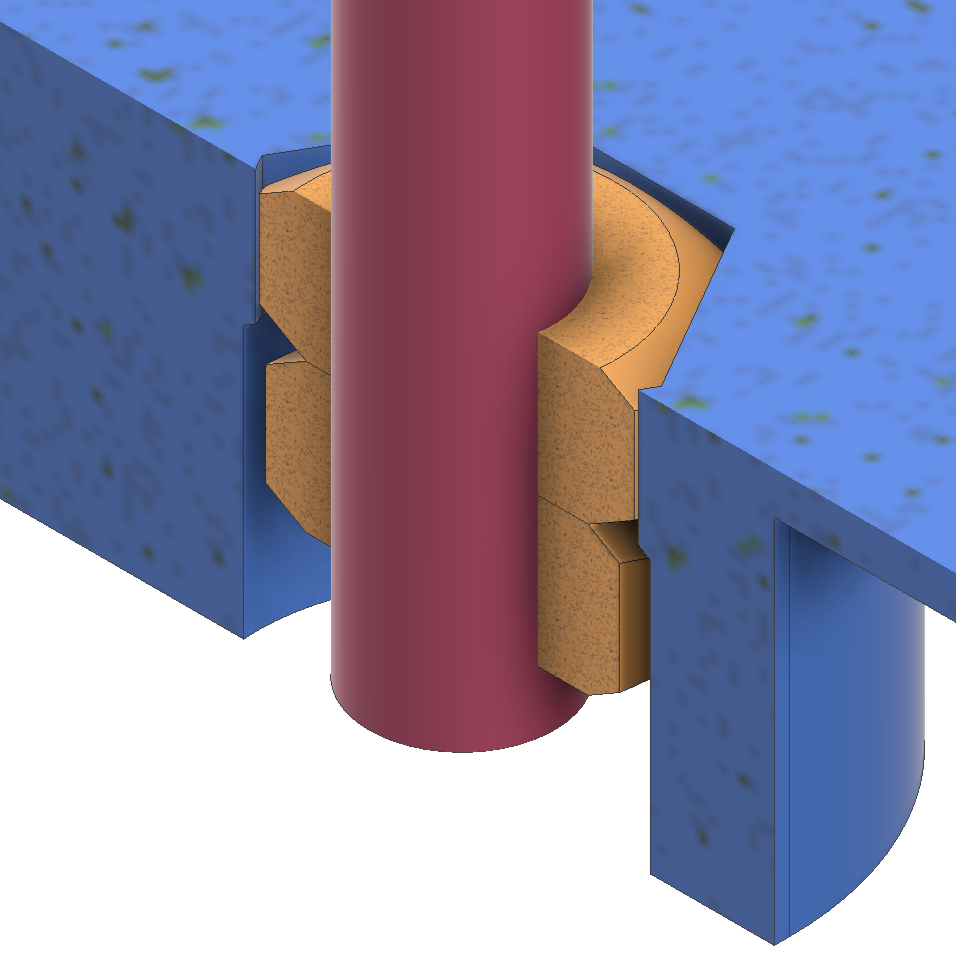
\includegraphics[width=.4\textwidth]{figures/InterlockingScrews.png}\label{fig:counterrotated}
    \caption{Counterrotated nuts.}
\end{figure}

\section{Elektronica ontwerp}
\section{Software ontwerp}

